\nonstopmode  % to allow pdflatex to compile even if errors are raised (e.g. missing figures)

\documentclass[10pt]{article}

\usepackage{amsmath}
\usepackage{amssymb}
\usepackage{bm}
\usepackage{graphicx}
% \graphicspath{{./figures/}} % save all figures in the same directory
\usepackage{color} 
\usepackage{hyperref}
\usepackage{parskip}
\setlength{\parindent}{0pt}

% Text layout
\topmargin 0.0cm
\oddsidemargin 0.5cm
\evensidemargin 0.5cm
\textwidth 16cm 
\textheight 21cm

%% PLEASE INCLUDE ALL MACROS BELOW
\newcommand{\etal}{\textit{et al.}} % use as "\etal{}" in citations
%\newcommand{\Prob}{\mathbb{P}} % symbol for proba
\newcommand{\Prd}{\mathsf{P}} % symbol for discrete proba
\newcommand{\Exp}{\mathbb{E}} % symbol for expectation
\newcommand{\Var}{\mathbb{V}} % symbol for variance
\newcommand{\Cov}{\mathbb{C}} % symbol for covariance
\newcommand{\Norm}{{\mathcal{N}}} % symbol for Normal distribution
\newcommand{\BF}{{\text{BF}}} % symbol for Bayes factor
\newcommand{\Lik}{{\mathcal{L}}} % symbol for likelihood
\newcommand{\bma}{{\BF_\text{BMA}}}
\newcommand{\bmalite}{{\BF_\text{BMAlite}}}
\newcommand{\av}{\mbox{\boldmath$\alpha$}}
\newcommand{\dv}{\bm{d}}
\newcommand{\der}{{\text{d}}} % "derivation" symbol inside integrals
\newcommand{\bv}{\mbox{\boldmath$\beta$}}
\newcommand{\tauv}{\mbox{\boldmath$\tau$}}
\newcommand{\cv}{\mbox{\boldmath$c$}}
\newcommand{\bbv}{\tilde \bv}
\newcommand{\bev}{\mbox{\boldmath$b$}}
\newcommand{\ev}{\mbox{\boldmath$e$}}
\newcommand{\thv}{\mbox{\boldmath$\theta$}}
\newcommand{\tv}{\mbox{\boldmath$t$}}
\newcommand{\fv}{\mbox{\boldmath$f$}}
\newcommand{\Cv}{\mbox{\boldmath$C$}}
\newcommand{\Dv}{\mbox{\boldmath$D$}}
\newcommand{\Fv}{\mbox{\boldmath$F$}}
\newcommand{\gav}{\mbox{\boldmath$\gamma$}}
\newcommand{\Gav}{\mbox{\boldmath$\Gamma$}}
\newcommand{\Kv}{\mbox{\boldmath$K$}}
\newcommand{\iv}{\mbox{\boldmath$I$}}
\newcommand{\vv}{\mbox{\boldmath$v$}}
\newcommand{\pv}{\mbox{\boldmath$p$}}
\newcommand{\hv}{\mbox{\boldmath$h$}}
\newcommand{\gv}{\mbox{\boldmath$g$}}
\newcommand{\wv}{\mbox{\boldmath$w$}}
\newcommand{\Wv}{\mbox{\boldmath$W$}}
\newcommand{\Pv}{\mbox{\boldmath$P$}}
\newcommand{\Qv}{\mbox{\boldmath$Q$}}
\newcommand{\Rv}{\mbox{\boldmath$R$}}
\newcommand{\rv}{\mbox{\boldmath$r$}}
\newcommand{\sv}{\mbox{\boldmath$s$}}
\newcommand{\Sv}{\mbox{\boldmath$S$}}
\newcommand{\Sigv}{\mbox{\boldmath$\Sigma$}}
\newcommand{\qv}{\mbox{\boldmath$q$}}
\newcommand{\Mv}{\mbox{\boldmath$M$}}
\newcommand{\mv}{\mbox{\boldmath$\mu$}}
\newcommand{\mvg}{\mbox{\boldmath$\mu_g$}}
\newcommand{\Lv}{\mbox{\boldmath$L$}}
\newcommand{\lav}{\mbox{\boldmath$\lambda$}}
\newcommand{\Tv}{\mbox{\boldmath$T$}}
\newcommand{\Xv}{\mbox{\boldmath$X$}}
\newcommand{\xv}{\mbox{\boldmath$x$}}
\newcommand{\Uv}{\mbox{\boldmath$U$}}
\newcommand{\Vv}{\mbox{\boldmath$V$}}
\newcommand{\yv}{\mbox{\boldmath$y$}}
\newcommand{\yvg}{\mbox{\boldmath$y_g$}}
\newcommand{\Yv}{\mbox{\boldmath$Y$}}
\newcommand{\Zv}{\mbox{\boldmath$Z$}}
\newcommand{\zv}{\mbox{\boldmath$z$}}
\newcommand{\lv}{\bf{1}}
\newcommand{\muLS}{\ensuremath{\hat{\mv}}}
\newcommand{\SigmaLS}{\ensuremath{\hat{\Sigma}}}
\newcommand{\fvPanel}{\ensuremath{\fv^{\rm panel}}}
\newcommand{\isa}{\ensuremath{\sigma_a^{-2}}}
\newcommand{\bfa}{\ensuremath{{\rm BF}}}
\newcommand{\hbfes}{\ensuremath{\widehat {\rm BF}^{\rm ES}}}
\newcommand{\hbfesmeta}{\ensuremath{\widehat {{\rm BF}}^{\rm ES}_{\rm meta}}}
\newcommand{\hbfesfix}{\ensuremath{\widehat {{\rm BF}}^{\rm ES}_{\rm fix}}}
\newcommand{\hbfesmax}{\ensuremath{\widehat {{\rm BF}}^{\rm ES}_{\rm maxH}}}
\newcommand{\hbfee}{\ensuremath{ \widehat {\rm BF}^{\rm EE} }}
\newcommand{\abfes}{\ensuremath{{\rm ABF^{ES}}}}
\newcommand{\abfee}{\ensuremath{{\rm ABF^{EE}}}}
\newcommand{\abfesc}{\ensuremath{{\rm A^*BF^{ES}}}}
%% END MACROS SECTION

\begin{document}

\title{Modeling Beyond the Configuration Model}
\author{Sarah Urbut}
\date{\today}

\maketitle

\tableofcontents

\vspace{1cm}

\section{Beyond the Config Model}

Recall that the Config Model made the following assumptions:

\section{Understanding the model}

Recall that for each tissue, we model the potential genetic association between a target SNP and the expression levels of a target gene by the simple linear regression model (\ref{simple.reg.model}). In vector form, this model is represented by
\begin{equation}
  \label{reg.model}
  \yv_r = \mu_r \lv + \beta_r \gv_r+ \ev_r,~\ev_r \sim \mathcal{N}(0,\sigma_r^2 I),
\end{equation}  

where $r$ indexes one of the $S$ tissue types examined and the vectors $\yv_r, \gv_r$ and $\ev_r$ denote the expression levels, the genotypes of the samples and the residual errors respectively for the $r^{\text{th}}$ tissue type.
The intercept term, $\mu_r$, and the residual error variance, $\sigma_r^2$ are allowed to vary with tissue type.
The regression coefficient $\beta_r$ denotes the effect of the eQTL in tissue $r$.

When the tissue samples are taken from the same individuals we allow that the observations on the same individual may be correlated with one another, but here I work with summary statistics and thus we assume that the residual errors among tissues.

Specifically, let $E := (\ev_1\,\cdots\,\ev_s)$  denote the $N \times R$ matrix of residual errors, the we assume it to follow a matrix-variate normal (MN) distribution, i.e.,
\begin{equation}
  E \sim {\rm MN}(0, I, \Sigma).
\end{equation}    
That is, the vectors $(\epsilon_{1i},\dots,\epsilon_{Ri})$ are independent and identically distributed as $\mathcal{N}(0, \Sigma)$.
The (unknown) $S \times S$ covariance matrix $\Sigma$ 
quantifies the correlations in the error between the $R$ tissues; it can vary from gene to gene and is estimated from the data (see below). In practice, we find that this matrix is close to diagonal, and again, when we work with summary statistics, we assume that the matrix of standard errors of $\hat\beta$, V_{gp} as approximated by $\hat{V_{gp}}$ is diagonal. 


But critically, the value of our method comes in considering the tissues jointly, and thus makes use of the multivariate vector of expression levels across all tissues.

Now, the likelihood for gene $g$ and SNP $p$ is:
\begin{equation}
Y_g | X_p, B_{gp}, X_c, B_{gc}, \Sigma_{gp} \sim \Norm_{N \times R}(X_p B_{gp} + X_c B_{gc}, I_N, \Sigma_{gp})
\end{equation}

where:
\begin{itemize}
\item $Y_g$ is the $N \times R$ matrix of expression levels;
\item $X_p$ is the $N \times 1$ matrix of genotypes (assuming the same individuals in all tissues);
\item $B_{gp}$ is the unknown $1 \times R$ matrix of genotype effect sizes;
\item $X_c$ is the $N \times (1+Q)$ matrix of known covariates (including a column of 1's for the intercepts);
\item $B_{gc}$ is the unknown $(1+Q) \times R$ matrix of covariate effect sizes (including the $\mu_s$);
\item $\Norm_{N \times R}$ is the \href{https://en.wikipedia.org/wiki/Matrix_normal_distribution}{matrix Normal distribution};
\item $\Sigma_{gp}$ is the unknown $R \times R$ covariance matrix of the errors.
\end{itemize}


For mathematical convenience (especially in the case of multiple SNPs), we vectorize the rows of $B_{gp}$ into $\bm{\beta}_{gp}$.
Here, as we focus on one SNP at a time, we directly have $\bm{\beta}_{gp} = B_{gp}^T$.

We use the notion of \emph{configuration}, a latent indicator $R$-dimensional vector $\bm{\gamma}_{gp}$ such that $\gamma_{gpr} = 1$ means the eQTL is active in tissue $r$, i.e. $b_{gpr} \ne 0$, whereas $\gamma_{gpr} = 0$ means the eQTL is inactive in tissue $r$, i.e. $b_{gpr} = 0$.
Moreover, we introduce an unknown mean $\bar{b}_{gp}$, to finally get the following ``spike-and-slab'' prior allowing to borrow information across tissues in which the eQTL is active:
\begin{equation}
  b_{gpr} | \gamma_{gpr}, \bar{b}_{gp}, \phi \sim \gamma_{gpr} \Norm(\bar{b}_{gp}, \phi^2) + (1 - \gamma_{gpr}) \delta_0
\end{equation}
where $\delta_0$ is a point mass at 0, and
\begin{equation}
  \bar{b}_{gp} | \omega \sim \Norm(0, \omega^2)
\end{equation}

 Thus if $\gamma_{gpr}=0$, then $\beta_{gpr}$ is by definition 0. Otherwise, the tissue specific variance is $\phi$. 
 
Whereas the configuration handles qualitative heterogeneity (having an effect or not), the hyperparameters $\phi$ and $\omega$ handles quantitative heterogeneity (having possibly different, non-null effects).
By integrating out $\bar{b}_{gp}$, we can see that $\phi^2 + \omega^2$ controls the average magnitude of the effect in any tissue  and $\phi^2/(\omega^2+\phi^2)$ controls the amount of heterogeneity.

Equivalently, we can write this prior as a multivariate Normal:
\begin{equation}
  \bm{b}_{gp} | U_{0} \sim \Norm_R(\bm{0}, U_{0})
\end{equation}

where, following Wen (2014), $U_{0}$ is parametrized as $(\Gamma_{gp},\Delta_{gp})$:
\begin{equation}
  p(U_{0}) = \Prd(\Gamma_{gp}) p(\Delta_{gp} | \Gamma_{gp})
\end{equation}
so that $\Gamma_{gp}$ is a binary matrix consisting of entry-wise non-zero indicators and is identical in size and layout to $U_{0}$, and $\Delta_{gp}$ is an indexed set of numerical values quantifying each non-zero entry in $\Gamma_{gp}$.
The skeleton $\Gamma_{gp}$ has $\bm{\gamma}_{gp}$ on the diagonal.
Each off-diagonal entry $\Gamma_{gp,ij}$ is equal to 1 has long as diagonal elements $\Gamma_{gp,ii}$ and $\Gamma_{gp,jj}$ are both equal to 1. Thus, for a configuration 1-0-1 for example, all the entries containing tissue 2 (i.e., the prior on the effect size covariances with tissue 2 and tissue 2's effect size variance) will be 0. Otherwise, 

In the current application, we choose:
\begin{equation}
  U_{0} \, | \, \bm{\gamma}_{gp} = \bm{1}, \phi, \omega \; \; =
  \begin{pmatrix}
    \phi^2 + \omega^2 & \cdots & \omega^2 \\
    \vdots & \ddots & \vdots \\
    \omega^2 & \cdots & \phi^2 + \omega^2
  \end{pmatrix}
\end{equation}
In terms of notation, the $0$ in $U_{0}$ indicates the prior.


In practice, we use a known grid for prior variances, i.e. $L$ pairs of values $(\phi_l,\omega_l)$ leading to a mixture of multivariate Normals:
\begin{equation}
  \label{prior_b_mixt_grid}
  \bm{b}_{gp} | \bm{\lambda},\Uv_0(\bm{\gamma}_{gp}) \sim \sum_{l=1}^L \lambda_l \; \Norm_R(\bm{0}, U_{0l}(\bm{\gamma}_{gp}))
\end{equation}
where $U_{0l}(\bm{\gamma}_{gp})$ indicates that the $U_{0l}$ matrix is a function of the configuration $\bm{\gamma}_{gp}$.

To simplify the notation, as there are $J=2^R-1$ active configurations, we now write $U_{0jl}$ for the prior covariance matrix for configuration $j$ and grid values $l$.
When combined with the prior on configurations, this leads to:
\begin{equation}
  \label{prior_b_mixt_grid_config}
  \bm{b}_{gp} | \bm{\eta},\bm{\lambda},\Uv_0 \sim \sum_{j=1}^J \eta_j \sum_{l=1}^L \lambda_l \; \Norm_R(\bm{0}, U_{0jl})
\end{equation}

Which leads us to a corresponding multivariate mixture posterior on $\bm{b}_{gp}$. 


\begin{equation}
\begin{aligned}
  \label{post_b_j_init}
p(\bm{b}_{gp} | \hat{\bm{b}}_{gp}, \hat{V}_{gp}, \hat{\bm{\lambda}}, \hat{\bm{\eta}}, v_{gp}=1) &= \sum_{l=1}^L \sum_{J=1}^J p(\bm{b}_{gpjl} | \hat{\bm{b}}_{gp}, \hat{V}_{gp}, c_{gpj}=1, d_{gpl}=1,v_{gp}=1) \\
&\times \Prd(d_{gpl}=1,c_{gpj}=1 | \hat{\bm{b}}_{gp}, \hat{V}_{gp}, \hat{\bm{\lambda} },\hat{\bm{\eta}},v_{gp}=1) 
\end{aligned}
\end{equation}

\section{Updates}

Now, suppose that instead of restricting ourselves to `fixed' $U_{0} $of the form: 

\begin{equation}
  U_{0} \, | \, \bm{\gamma}_{gp} = \bm{1}, \phi, \omega \; \; =
  \begin{pmatrix}
    \phi^2 + \omega^2 & \cdots & \omega^2 \\
    \vdots & \ddots & \vdots \\
    \omega^2 & \cdots & \phi^2 + \omega^2
  \end{pmatrix}
\end{equation}

We allow our estimate of $U_{0}$ to be informed by the data. Specifically, let us imagine modeling the prior on the covariance of effects as a linear combination of the effects in each tissue, such that we can imagine a covariance matrix that reflects a linear combination of `stretches' along axes defined by standardized effects in each tissue.  In the univariate case, ash assumes that all $\beta_{j}$ come from some shared mixture distribution where the proportion of each component is 'learned' from the data by maximizing the likelihood across all gene SNP pairs. Now, each $\bm{b}_{j}$ is actually a vector of effect sizes across tissues for a given gene-snp pair, and so we simply make the assumption that this shared distribution from which all $\bm{b}_{j}$ arise is a mixture of multivariate normals, with each of the $K$ multivariate normals specified by the prior covariance matrix for $\bm{b}$, $U_{k}$.


In selecting these prior covariance matrices $U_{k}$, we can 'learn' these covariance matrices from the data, or specify a fixed set of covariance matrices from which we learn the relative weight, similar to the methods above. We will begin by modeling the prior on $\beta_{gp}$ as descending from a mixture of multivariate normals, using a learned combination of weighted covariance matrix of the t statistics, and the first $K$ factors of the Sparse Factor Representation. Importantly, learning across gene-snp pairs $j$ also allows us to share information across tissues, if we learn the proportion descending from a component which puts heavy weight on a shared effect (as in the fixed effect case).




\begin{figure}[h]
    \includegraphics[scale=0.5]{SFApic.pdf}
\end{figure}

\section{Understanding SFA}

Both PCA and SFA attempt to approximate each tissues' $\beta_{i,..p}$ vector by a linear combination of $\beta_{i,..p}$ across tissues. 

In SFA, at gene-snp pair $j$ in tissue 1, tissue 1 will have loading on only the first factor, which represents the direction of effect in tissue 1, $\beta_{1,j}$. Similarly, we can see that F[1,1] results from L[,1] * G[,1] and so if L[,1] (the first loading, with coordinates for each tissue) is a vector of
\begin{pvector}
 [1 0 0 .. R]
 \end{pvector}
 
 Then the corresponding Factor will receive only input from $\beta_{1,J}$ and thus can be thought of the direction corresponding to effect in tissue 1. The entire vector $F[1,]$ can then be thought of the pointing in the direction of 'true' effect over all gene SNP pairs for tissue 1, and F[2,] can be thought of the direction of effect across all genes in tissue 2, etc.  But  because tissue 1 $\beta_{j}$ will have loading only on $F[1,]$, the predicted gene expression in tissue 1 will simply be the $\beta_{j1}$ for tissue 1 at each of the J gene-snp pairs. By contrast, the first factor of PCA will be a weighted average of $\beta_{j1..R}$ across all tissues for a given gene-snp pair $j$, because each tissue $\beta$ will receive equal loading since there is no requirement that the column sum of L be 1. Thus in PCA, each of the $j$ elements of each factor $F[,k]=[1..j]$ represent a linear combination of the effect size of $\beta_{j}$ across all tissues, while in sparse factor analysis they represent only the effect in $\beta_{k}$. Similarly, the loadings in PCA represent linear combinations of the $j$ genes for each of the $n$ individuals, while in factor analysis they can be more appropriately thought of as the relative importance of a particular factor (here, vector of effects in one tissue) on that sample. Since in practice we do not observe the true $\beta_{jl}$ and are thus attempting to make an inference from the observed $\hat{\beta_{j}$, we will instead use the $R$ x $P$ matrix of t statistics.
 
 
 
\subsection{Visualization}
\begin{itemize}
\item Think of the 'Factors" as corresponding to the direction of effect for tissue 1...R across all $p$ SNPs. Along the same lines of thinking as Ash, we can actually assume that there are `shared' patterns of effect in tissue 1 across all $j$ gene-snp pairs, such that this direction can probably be specified by a reduced set of gene-snp Pairs (in fact, the maximal number of linearly independent columns must be R, if R<<P).
\item If we say that all vectors $\bm\b_{j}$ `share' information, we can estimate them from the same multivariate normal distribution. In fact, we use a mixture of multivariate normals, which is estimated hierarchically by finding the optimal combination of distributions to maximize the likelihood across all gene-snp pairs. Thus if some gene-snp pairs tend to exhibit stronger `effects' in tissue 1, they will push the weight $\pi_{k,l}$ corresponding to a large prior variance for $\bm{b}_{1}$ up, while if most `gene-snp' pairs show similar large effects in all tissues, then  the $\pi_{k,l}$ might be very similar when $\omega_{l}$ is large, if we allow each of the $U_{k,l}$ matrices to represent the $L[,k] L[,k]^{t}$ matrix. That is, the matrix quantifying the loadings of 'eigentissue K' for each tissue, or equivalently, a weighted combination of all-gene SNP pairs' characteristic pattern K expression.
\item We can thus form a mixture of multivariate normals, from which each unobserved $\bm\b_{j}$ multivariate vectors is expected to lie. In the univariate case, the variance specifies the `width' of this distribution along the 'tissue 1' axis, for example, where the tissue 1 axis can be thought of as a summary of the direction of behavior of all $j$ end snp pairs in tissue 1. Now, we add an additional tissue 2 axis, which is similarly constructed as a summary of behavior of all $j$ gene-snp pairs in tissue 2 (i.e., each of the $j$ elements of this vector corresponds to the ideal activity in tissue $k$ at gene snp pair $j$, thus the axis is itself $j$ dimensional). The prior covariance term just specifies the width of the ellipse formed by the covariance between these two distribution for every mixture component - i.e., how well does activity in tissue 1 for $\beta_{j1}$ correspond to activity in tissue 2 for $\beta_{j2}$.
\item You can see that in SFA, the loadings result from a linear combination of the genes, and the factors result from a linear combination of the individuals. So for v[1,1] (or equivalently L[1,k] expresses how much of eigen tissue 'k' individual 1 contains across the `optimal' combination of genes. It us the 'eigengen' because it represent a summary of `k'ness across the genome.
\item If we know that in SVD, the Us result from linear combination of the individuals while the Vs result from a linear Combination. In PCA, the first factor might represent the genomic profile of an 'average individual' at each gene, then in Factor Analysis it simply represents 'individual 1' type eigenarray (i.e., the expression of tissues most similar to group 1 in our example across the whole genome). Thus the 'linear combination' would put no weight on the contribution of the genomic profile fromother tissue types, and all weight on samples of tissue type 'k'. The Vs are linear combinations of the columns of U^{t} and similarly, each element of V[,k] represents a linear combinations of the features of an individual. Thus in PCA, it might represent the amount of 'average' individual he features across his genome, while in Factor Analysis it represents how much 'individual 1' he features across his genome. It makes sense, then, that you can represent the covariance matrix of individuals as $VV^{t}$, because each $V^{k}$ is a genomic summary of every individual, while the true Covariance Matrix X^{t}X is compares individuals as well, but element by element.
\item We can think of the loadings as how much eigentissue k an individual has across the genome. Equivalently, F[k,1]  equals how much 'eigengene1' this gene contains across all individuals. Effectively these 'eigengenes' and 'eigentissue' really represent eigen patterns which separate individuals (and genes) into how well each captures a particular pattern. For example, suppose Factor 1 corresponded to the ideal expression for eigenpattern 1. Than the values in each of the $p$ elements of F1 would represent the 'loadings' of that feature on the 'eigenpattern' - e.g., how much that gene contributes to eigenpattern1. Equivalently, the loadings in L[1] represent how much that individual contains eigenpattern1.
\item The reason that we will use L[,k]*L[,k]' to approximate the covariance matrix of V is because 

\begin{equation}
X_{rxp}=L_{rxk}F_{kxp}\\ 
X_{rxp}X_{rxp}^{t} \approx \frac{1}{P} LF F'L'\\
&\approx L_{k} L_{k}'

\begin{figure}[h]
    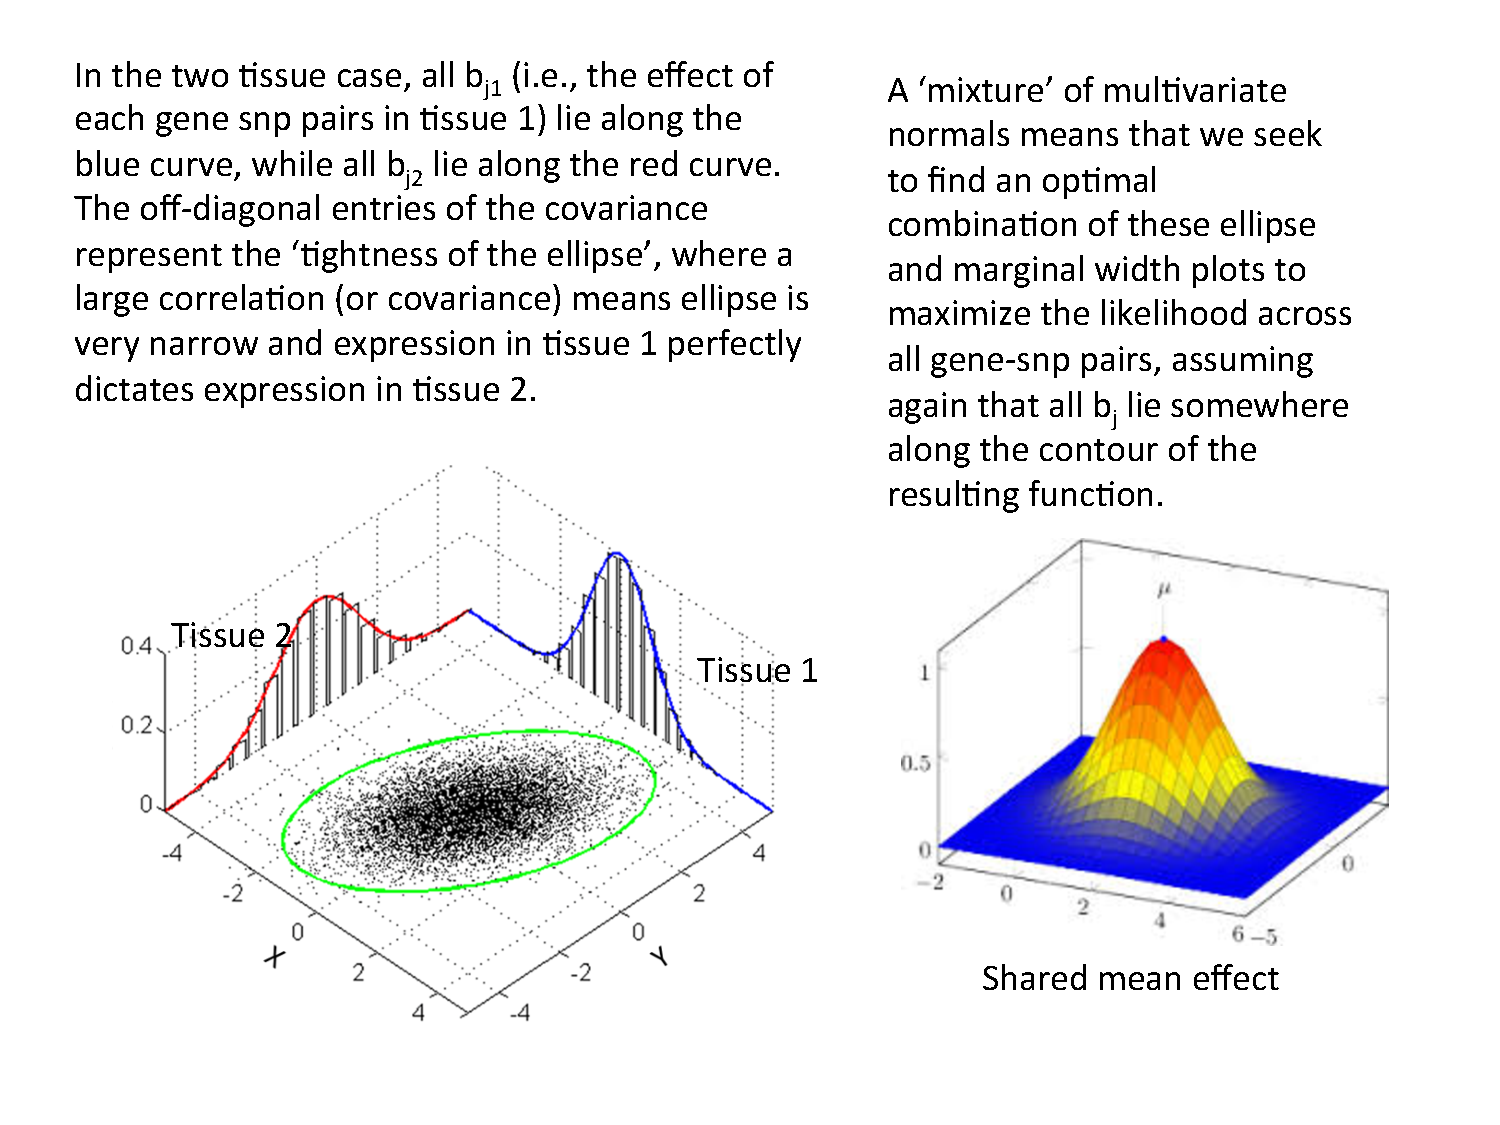
\includegraphics[scale=0.5]{multidensity.pdf}
\end{figure}

 \section{General Algorithm}
 
 For all $j$  gene-snp pairs, beta $\bm{b}_{j}$ represent the unknown standardized effect of a snp `p' on gene 'g'. 
 
 \begin{equation}
  \label{prior_b_mixt_grid}
  \bm{b}_{j} | \bm{\pi},\Uv_0 \sim \sum_{k,l} \pi_{k,l} \; \Norm_R(\bm{0}, \omega^{2}_l U_{k})
\end{equation}

As mentioned, we can `learn' $U_{k}$ from the data or specify each $U_{k}$ and learn the relative proportion of each mixture component from the data via the EM algorithm. 

In the special case where K = 1, as a first proposal for $U_{k}$ when $R$ is small, we let $\bm{t}_{r}$ represent the vector of $t$ statistics across all $j$ gene-snp pairs in tissue $r$. and $\mu_{r}$ represent the mean t statistic across all $j$ gene-snp pairs in tissue $r$.

\begin{equation}
  U_{0} \, |  \omega \; \; =
  \begin{pmatrix}
 \omega^2 \ (\bm{t}_{r} - \mu_{r}) (\bm{t}_{r} - \mu_{r})^{t} & \cdots & \omega^2 (\bm{t}_{r} - \mu_{r}) (\bm{t}_{r'} - \mu_{r'})^{t} \\
    \vdots & \ddots & \vdots \\
    \omega^2 (\bm{t}_{r} - \mu_{r}) (\bm{t}_{r'} - \mu_{r'})^{t} & \cdots &\omega (\bm{t}_{r'} - \mu_{r'}) (\bm{t}_{r'} - \mu_{r'})^{t} 
  \end{pmatrix}
\end{equation}

Here, we pre-specify $\omega^{2}_{l}$ \in [0,0.01,0.02 ...]$ where each $\omega^{2}$ can be though of as a 'stretch' along the vector corresponding to each factor. (But what is the connection between the factors and the prior covariance matrix? Or the covariance matrix of t statistics).

Similarly, can let $U_{k}$ = $\bm{\gamma}_{k} \bm{\gamma_{k}}^{t}$ where $\bm{\gamma_{k}}$ represents the $R$ by $1$ vector corresponding to the `kth' loading from the Sparse Factor representations of the covariance matrix of t statistics, which summarize behavior of all $t_{j}$ in tissue {1..k}$ respectively. 

\section{EM Algorithm Outline}
Given these $U_{k}$, we can now obtain MLEs for $\pi_{kl}$ by a simple EM algorithm, in which we seek to choose the `optimal' combination of covariance matrices $\U_{k}$ from which to model the posterior distribution of $\beta_{j}$. 

We will use the following algorithm:

1) For each prior covariance matrix $U_{k}$ and `stretch' factor $\omega_{l}$ compute 


\begin{equation}
\begin{aligned}
L (\beta_{j};k,l) = \Pr(\hat{\bm{b}_{j}} | k,l) \\
&= \Pr(\hat{\bm{b}_{j}}; 0, \omega^{2}_{l} U_{k} + \hat {V})

\end{aligned}
\end{equation}

Then, we can set 
\begin{equation}
w_{jkl} = \frac{\pi_{k,l} L(\beta_{j};k,l)}{\sum_{k,l} \pi_{k,l} L(\beta_{j};k,l)}
\end{equation}

We can then update our estimate of $\pi_{k,l}$ as 

\begin{equation}
\pi_{kl}^{i+1} = \frac{\sum_{j} w_{jkl}}{\sum_{j,k,l} w_{jkl}}
\end{equation}

Which amounts to iteratively updating the weights such that they maximize the likelihood of the data across all gene snp pairs, assuming all vectors $\beta_{j}$ arise from some shared mixture distribution and thus inform our estimates of each $\beta_{j}$. We can begin with $U_{0}$ = I, $U_{1} = \hat{\Sigma}$ where $\hat{\Sigma}$ represents the estimated RxR covariance matrix of T statistics, and $U_{2}$ is $U_{k{i,j}}$ as $F_{i} \dot F_{j}^{t}$, which, if we assume the $F_{k}$ are broadly capturing direction of effect across genes in tissue 1..R and there are at most k=R factors, then each element {i,j} of $U_{k}$ is the factor corresponding to the covariance between tissue $i$ and tissue $2$ in the case of the approximated covariance matrix. 

In order to determine the hierarchical weight that separates the relative importance of one tissue expression pattern, we will separate each of the U_{k} rather than using the sum of the first K (as you suggested in the $VV'{t}$ example). In the F ~ I case, each $U_{k}$ (approximated covariance matrix) will then be derived from the loadings on tissue-specific K expression profile for each tissue. Each element of $U_{k}$ will then represent the covariance of tissue $r_{i}$ and $r_{j}$ based on their loadings on this expression profile.


\end{document}
